\documentclass{article}
\usepackage{amsmath}
\usepackage{amssymb}
\usepackage[a4paper, top=25mm, bottom=25mm, left=25mm, right=25mm]{geometry}
\usepackage{pgfplots}
\usepackage{mathtools}
\usepgfplotslibrary{fillbetween}
\pgfplotsset{compat=1.18}

\begin{document}
\pagestyle{empty}
\large

\begin{center}
2024-2025 Fall \\MAT123-02,05 Makeup\\(31/01/2025)
\end{center}

\noindent 1.

\hfill

\noindent (a) Find $\displaystyle\int\frac{\sin^3x}{\sqrt{\cos x}}\,dx$.

\hfill

\hfill

\noindent (b) Find $\displaystyle\int\frac{dx}{x^3-4x^2+3x}$.

\hfill

\hfill

\noindent (c) Evaluate $\displaystyle\lim_{x\to\textstyle\frac\pi2}\frac{\displaystyle\int_{\pi/2}^x\ln(\sin t)\,dt}{\sin x-1}$.

\hfill

\hfill

\noindent (d) Evaluate the improper integral $\displaystyle\int_0^2\frac{dx}{(x-1)^{2/3}}$.

\hfill

\hfill

\noindent 2. Consider the region $R$ bounded by the curves $y=\arctan x,\:y=\ln x$ and the lines $\displaystyle x=\frac1{\sqrt3}$ and $x=1$.

\hfill

\noindent (a) Sketch the region and find the area of the $R$. 

\hfill

\noindent (b) Write a definite integral (do not evaluate) by using the Washer Method, which gives the volume of a solid obtained by rotating the region $R$ about the $y$-axis.

\hfill

\noindent (c) Write a definite integral (do not evaluate) by using the Cylindrical Shell Method, which gives the volume of a solid obtained by rotating the region $R$ about the line $y=2$.

\hfill

\noindent 3. Determine whether each series is convergent or divergent. Explain your answer.

\hfill

\noindent (a) $\displaystyle\sum_{n=0}^\infty\frac{(-3)^{n+1}}{2^{3n}}$

\hfill

\noindent (b) $\displaystyle\sum_{n=2}^\infty\frac1{n(\ln n)^2}$

\hfill

\noindent 4. Find the Taylor series of the function $f(x)=\ln x$ at $c=1$ and determine the interval of convergence.

\newpage

\begin{center}
2024-2025 Makeup (31/01/2025) Solutions\\
(Last update: 17/08/2025 20:56)
\end{center}

\noindent 1.

\hfill

\noindent (a)
\[\int\frac{\sin^3x}{\sqrt{\cos x}}\,dx=\int\frac{\left(1-\cos^2x\right)\cdot\sin x}{\sqrt{\cos x}}\,dx\]

\hfill

\noindent Let $u=\cos x$, then $du=-\sin x\,dx$.

\begin{align*}\int\frac{\left(1-\cos^2x\right)\cdot\sin x}{\sqrt{\cos x}}\,dx&=\int-\frac{\left(1-u^2\right)}{\sqrt{u}}\,du=\int\left(u^{3/2}-\frac1{\sqrt u}\right)=\frac25u^{5/2}-2\sqrt u+c\\\\&=\boxed{\frac25\left(\cos x\right)^{5/2}-2\sqrt{\cos x}+c,\quad c\in\mathbb{R}}\end{align*}

\hfill

\noindent (b) Use the method of partial fraction decomposition.

\[\int\frac{dx}{x^3-4x^2+3x}=\int\frac{dx}{x(x-3)(x-1)}=\int\left(\frac Ax+\frac B{x-3}+\frac C{x-1}\right)\,dx\]

\[\begin{array}{rc}A(x-3)(x-1)+Bx(x-1)+Cx(x-3)&=1\\x^2(A+B+C)+x(-4A-B-3C)+3A&=1\\&\end{array}\]

\hfill

\noindent Equate the coefficients of like terms.

\[\left.\begin{array}{r}
x^2(A+B+C)=0\\
x(-4A-B-3C)=0\\
3A=1
\end{array}\right\}\rightarrow A=\frac13,\qquad\left.\begin{array}{r}
B+C=-\dfrac13\\[1em]
B+3C=-\dfrac43
\end{array}\right\}\rightarrow B=\frac16,\quad C=-\frac12\]

\hfill

\noindent Rewrite the integral.

\begin{align*}
\int\left(\frac Ax+\frac B{x-3}+\frac C{x-1}\right)\,dx&=\int\left(\frac1{3x}+\frac1{6(x-3)}-\frac1{2(x-1)}\right)\,dx\\\\&=\boxed{\frac13\ln|x|+\frac16\ln|x-3|-\frac12\ln|x-1|+c,\quad c\in\mathbb{R}}
\end{align*}

\hfill

\noindent (c) The limit is in the indeterminate form $0/0$. Apply L'Hôpital's rule to eliminate the indeterminate form.

\[\lim_{x\to\textstyle\frac\pi2}\frac{\displaystyle\int_{\pi/2}^x\ln(\sin t)\,dt}{\sin x-1}\overset{\text{L'H.}}{=}\lim_{x\to\textstyle\frac\pi2}\frac{\displaystyle\frac d{dx}\int_{\pi/2}^x\ln(\sin t)\,dt}{\cos x}\]

\hfill

\noindent By the Fundamental Theorem of Calculus, we may rewrite the limit as follows.

\begin{align*}\lim_{x\to\textstyle\frac\pi2}\frac{\displaystyle\frac d{dx}\int_{\pi/2}^x\ln(\sin t)\,dt}{\cos x}&=\lim_{x\to\textstyle\frac\pi2}\frac{\ln(\sin x)}{\cos x}\overset{\text{L'H.}}{=}\lim_{x\to\textstyle\frac\pi2}\frac{\frac1{\sin x}\cdot\cos x}{-\sin x}=\lim_{x\to\textstyle\frac\pi2}\frac{\cos x}{-\sin^2x}=-\frac{\cos\frac\pi2}{\sin^2\frac\pi2}\\\\&=\boxed0\end{align*}

\hfill

\noindent (d) Take the limit as this is an improper integral.

\begin{align*}\int_0^2\frac{dx}{(x-1)^{2/3}}&=\lim_{R\to1^-}\int_0^R\frac{dx}{(x-1)^{2/3}}+\lim_{P\to1^+}\int_P^2\frac{dx}{(x-1)^{2/3}}\\\\&=\lim_{R\to1^-}3(x-1)^{1/3}\Bigg|_0^R+\lim_{P\to1^+}3(x-1)^{1/3}\Bigg|_P^2\\\\&=3\lim_{R\to1^-}\left((R-1)^{1/3}-(-1)\right)+3\lim_{P\to1^+}\left(1-(P-1)^{1/3}\right)=\boxed6\end{align*}

\hfill

\noindent 2.

\hfill

\noindent (a)
\begin{center}
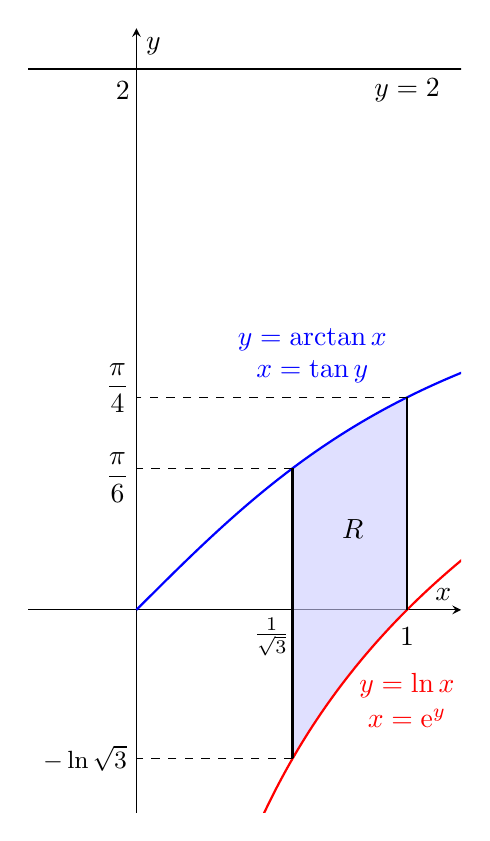
\begin{tikzpicture}
  \begin{axis}[
      axis lines=center,
      axis equal image,
      xlabel={$x$},
      ylabel={$y$},
      xmin=-0.4, xmax=1.2,
      ymin=-0.75, ymax=2.15,
      samples=200,
      scale=1.75,
      domain=0.577:1,
      xtick=\empty, ytick=\empty,
    ]

    \addplot [thick, blue, name path=A, domain=0:2] {rad(atan(x))};
    \addplot [thick, red, name path=B, domain=0.1:2] {ln(x)};
    \addplot [blue!20, fill opacity=0.6] fill between[of=A and B,soft clip={domain=0.577:1}];
    
    \draw[dashed] (-3,0) -- (-3,3); \draw[dashed] (-3,3) -- (-0.5,3);
    \draw[dashed] (2,0) -- (2,8); \draw[dashed] (0,8) -- (2,8);

    \node[blue] at (0.65,1) {$y=\arctan x$}; \node[blue] at (0.65,0.88) {$x=\tan y$};
    \node[red] at (1,-0.28) {$y=\ln x$}; \node[red] at (1,-0.4) {$x=\mathrm{e}^y$};

    \draw[thick] (0.577,-0.549)--(0.577,0.523); \draw[thick] (1,0)--(1,0.785);
    \draw[dashed] (1,0.785)--(0,0.785); \draw[dashed] (0.577, 0.523)--(0,0.523);
    \draw[dashed] (0.577,-0.549)--(0,-0.549);
    \draw[thick] (-1,2)--(2,2); 
    
    \node at (0.8,0.3) {$R$}; \node at (0.5,-0.1) {$\frac1{\sqrt3}$}; \node at (-0.07,0.49) {$\dfrac\pi6$}; \node at (-0.07,0.82) {$\dfrac\pi4$}; \node at (-0.19,-0.549) {\small $-\ln\sqrt3$}; \node at (1,-0.1) {$1$}; \node at (-0.05,1.92) {$2$}; \node at (1,1.92) {$y=2$};
\end{axis}
\end{tikzpicture}
\end{center}

\begin{equation}A=\int_{1/\sqrt3}^1\left(\arctan x-\ln x\right)\,dx=\int_{1/\sqrt3}^1\arctan x\,dx-\int_{1/\sqrt3}^1\ln x\,dx\end{equation}

\hfill

\noindent Calculate the first integral in $(1)$ by integration by parts.

\[\left.\begin{array}{c}
u=\arctan x\implies du=\dfrac1{x^2+1}\,dx\\[1em]
dv=dx\implies v=x
\end{array}\right\}\rightarrow \int u\,dv=uv-\int v\,du\]

\begin{align*}\int_{1/\sqrt3}^1\arctan x\,dx&=x\arctan x\bigg|_{1/\sqrt3}^1-\int_{1/\sqrt3}^1\frac{x}{x^2+1}\,dx=\left(x\arctan x-\frac12\ln\left|x^2+1\right|\right)\Bigg|_{1/\sqrt3}^1\\\\&=\left(\frac\pi4-\frac{\ln 2}2\right)-\left(\frac{\pi\sqrt3}{18}-\frac12\cdot\ln\left(\frac43\right)\right)=\frac{\pi\left(9-2\sqrt3\right)}{36}+\frac12\cdot\ln\frac23\end{align*}

\hfill

\noindent Calculate the second integral in $(1)$ by integration by parts.

\[\left.\begin{array}{c}
u=\ln x\implies du=\dfrac1x\,dx\\[1em]
dv=dx\implies v=x
\end{array}\right\}\rightarrow \int u\,dv=uv-\int v\,du\]

\begin{align*}\int_{1/\sqrt3}^1\ln x\,dx&=x\ln x\bigg|_{1/\sqrt3}^1-\int_{1/\sqrt3}^1\,dx=\left(x\ln x-x\right)\Bigg|_{1/\sqrt3}^1=\left(0-1\right)-\left(-\frac{\ln\sqrt3}{\sqrt3}-\frac1{\sqrt3}\right)\\\\&=\frac{\sqrt3\ln\sqrt3+\sqrt3-3}3\end{align*}

\hfill

\noindent The result is then

\[A=\boxed{\frac{\pi\left(9-2\sqrt3\right)}{36}+\frac12\cdot\ln\frac23-\frac{\sqrt3\ln\sqrt3+\sqrt3-3}3}\]

\hfill

\noindent (b)
\begin{align*}\boxed{\begin{array}{l}\displaystyle\int_{-\ln\sqrt3}^0\pi\left[\left(\mathrm{e}^y\right)^2-\left(\frac1{\sqrt3}\right)^2\right]\,dy+\int_0^{\pi/6}\pi\left[(1)^2-\left(\frac1{\sqrt3}\right)^2\right]\,dy\\\\\displaystyle+\int_{\pi/6}^{\pi/4}\pi\left[(1^2)-\left(\tan y\right)^2\right]\,dy\end{array}}\end{align*}

\hfill

\noindent (c)
\begin{align*}\boxed{\begin{array}{l}\displaystyle\int_{-\ln\sqrt3}^02\pi\left(2-y\right)\left(\mathrm{e}^y-\frac1{\sqrt3}\right)\,dy+\int_0^{\pi/6}2\pi\left(2-y\right)\left(1-\frac1{\sqrt3}\right)\,dy\\\\\displaystyle+\int_{\pi/6}^{\pi/4}2\pi\left(2-y\right)\left(1-\tan y\right)\,dy\end{array}}\end{align*}

\hfill

\noindent 3.

\hfill

\noindent (a)
\[\sum_{n=0}^{\infty}\frac{(-3)^{n+1}}{2^{3n}}=\sum_{n=0}^{\infty}\frac{-3\cdot(-3)^n}{8^n}=-3\sum_{n=0}^{\infty}\left(-\frac38\right)^n\]

\hfill

\noindent This is a geometric series where $r=-\dfrac38$. $|r|=\dfrac38<1$. Therefore, the series $\displaystyle\sum_{n=0}^{\infty}\frac{(-3)^{n+1}}{2^{3n}}$ converges.

\hfill

\noindent (b) Take $\displaystyle f(x)=\frac1{x(\ln x)^2}$. $f$ is positive and decreasing for $x\geq2$ because $x$ and $(\ln x)^2$ are positive and increasing for $x\geq2$. $x$ is a polynomial which is defined everywhere and $(\ln x)^2$ is continuous for $x\geq2$. Since we took into account every criterion, we may apply the Integral Test. Handle the improper integrals by taking the limit.

\[\int_2^{\infty}\frac{dx}{x(\ln x)^2}=\lim_{R\to\infty}\int_2^R\frac{dx}{x(\ln x)^2}=\lim_{R\to\infty}\left[-\frac1{\ln x}\right]_2^R=\lim_{R\to\infty}\left[-\frac1{\ln R}+\frac1{\ln2}\right]=\frac1{\ln 2}\]

\hfill

\noindent Since the integral converges, the series $\displaystyle\sum_{n=2}^\infty\frac1{n(\ln n)^2}$ also converges.

\hfill

\noindent 4. The Taylor series of $f$ at $c=1$ is as follows.

\[\sum_{k=0}^{\infty}\frac{f^{(k)}(1)}{k!}(x-1)^k\]

\hfill

\noindent Find $f(1),\:f'(1),\:f''(1),\:f'''(1)\:f^{(4)}(1)$ to look for the pattern.

\[f'(x)=\frac1{x},\quad f''(x)=-\frac1{x^2},\quad f'''(x)=\frac2{x^3}\quad f^{(4)}(x)=-\frac6{x^4} \]

\[f(1)=0,\quad f'(1)=1,\quad f''(1)=-1,\quad f'''(1)=2,\quad f^{(4)}(1)=-6\]

\hfill

\noindent This is an alternating sequence where the coefficient of each term is the factorial of the subsequent number starting from $0$ except for $k=0$, that is, the first term of the series. At $k=0$, the first term is $0$. So,

\[f^{k}(1)=\left\{\begin{array}{ll}(-1)^{k-1}\cdot (k-1)!,&\text{if}\: k>0\\0,& \text{if}\:k=0\end{array}\right.\]
\begin{align*}\sum_{k=0}^{\infty}\frac{f^{(k)}(1)}{k!}x^k&=0+\sum_{k=1}^{\infty}\frac{f^{(k)}(1)}{k!}(x-1)^k=\sum_{k=1}^{\infty}\frac{(-1)^{k-1}\cdot(k-1)!}{k\cdot(k-1)!}(x-1)^k\\\\&=\boxed{\sum_{k=1}^{\infty}\frac{(-1)^{k-1}\cdot(x-1)^k}{k}=(x-1)-\frac{(x-1)^2}2+\frac{(x-1)^3}3-\frac{(x-1)^4}4+...}\end{align*}

\hfill

\noindent Now, determine the interval of convergence. Apply the Ratio Test.

\begin{align*}\lim_{k\to\infty}\left|\frac{(-1)^k(x-1)^{k+1}}{k+1}\cdot\frac{k}{(-1)^{k-1}(x-1)^k}\right|&=\lim_{k\to\infty}\left|\frac{(x-1)\cdot k}{(k+1)\cdot(-1)}\right|=|x-1|\lim_{k\to\infty}\left|\frac k{k+1}\right|\\\\&=|x-1|\end{align*}

\[|x-1|<1\implies-1<x-1<1\implies0<x<2\quad(\text{convergent})\]

\hfill

\noindent Investigate the convergence at the endpoints.

\[x=0\rightarrow\sum_{k=1}^{\infty}\frac{(-1)^{k+1}\cdot(-1)^k}{k}=\sum_{k=1}^{\infty}\frac{(-1)^{2k}\cdot(-1)}{k}=-\sum_{k=1}^{\infty}\frac{1}{k}\]

\hfill

\noindent This is a $p$-series with $p=1$, for which the series diverges by the $p$-series Test. Try $x=2$.

\[x=2\rightarrow\sum_{k=1}^{\infty}\frac{(-1)^{k+1}}{k}\]

\hfill

\noindent This is an alternating series. The non-alternating part, which is $\frac1k$, is nonincreasing for $k\geq1$ and it is positive. The limit at infinity is $0$. By Leibniz's Alternating Series Test, the series converges.

\hfill

\noindent The convergence set for the power series is $\boxed{(0,2]}$.

\end{document}